\chapter{Results}%
\label{cha:results}


\section{Toy Example}%
\label{sec:toy_example}

\begin{figure}[htpb] \centering
    \begin{subfigure}[]{0.4\textwidth}
        \centering
    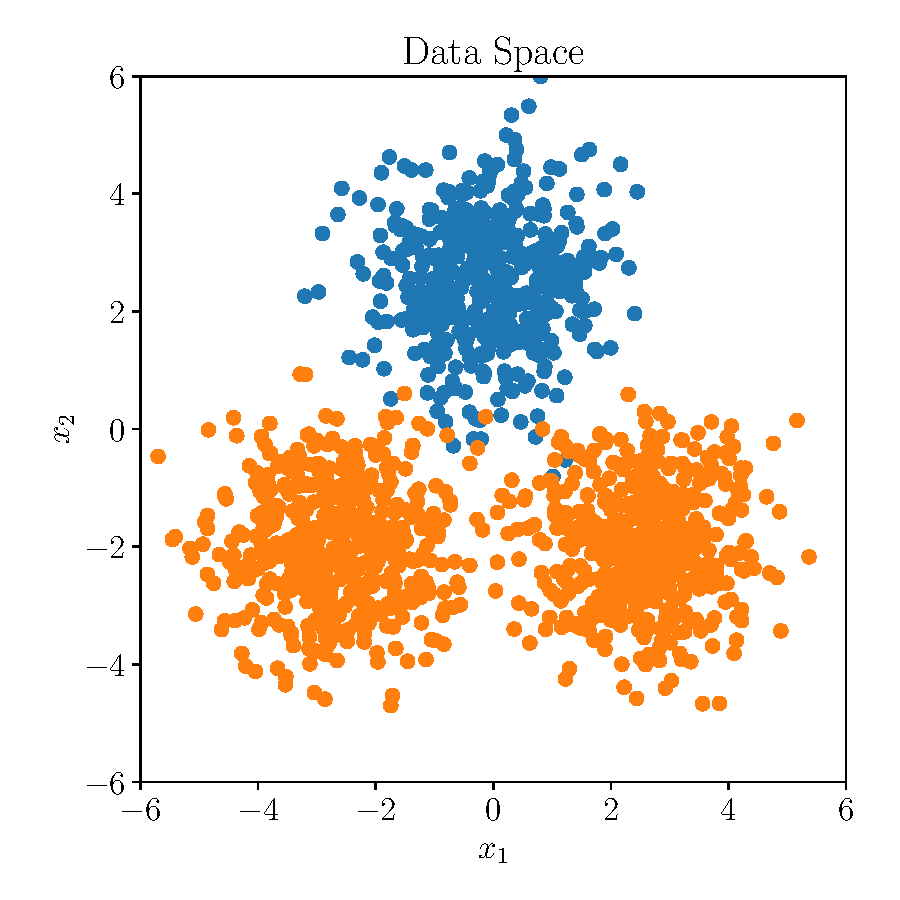
\includegraphics[width=\linewidth]{figures/toy_example/gaussian_mixture/toy_data.pdf}
        \caption{Test}
        \label{fig:gmm_sample_space}
    \end{subfigure}
    \begin{subfigure}[]{0.4\textwidth}
        \centering
    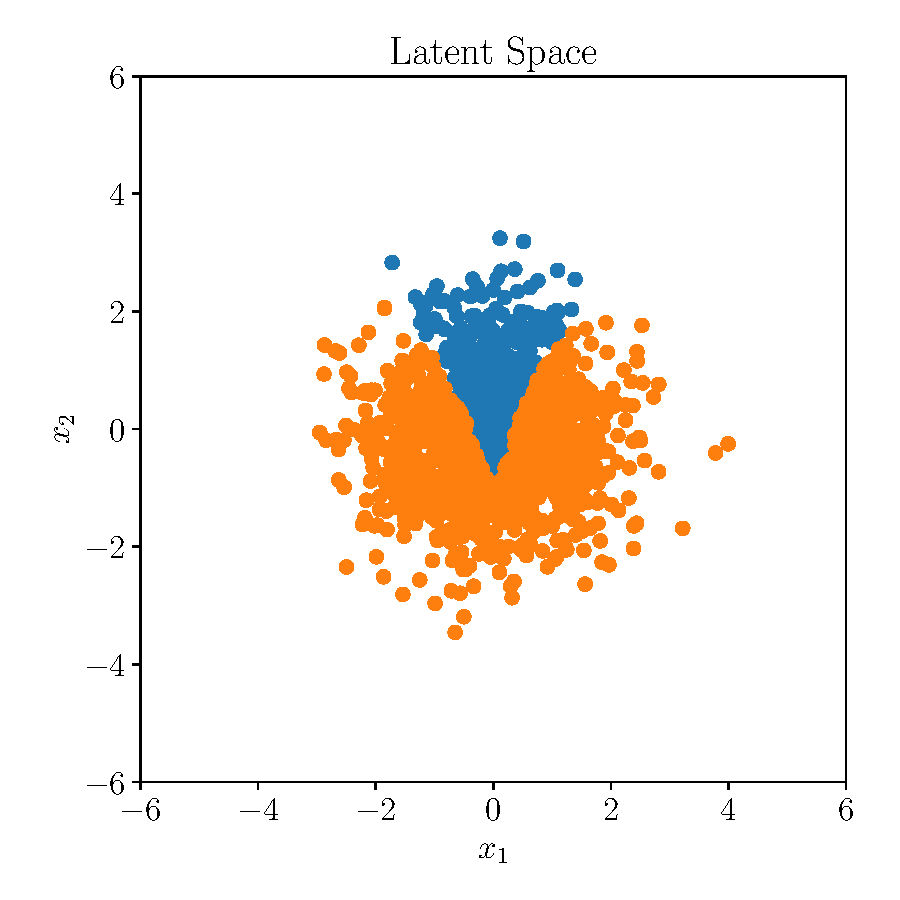
\includegraphics[width=\linewidth]{figures/toy_example/gaussian_mixture/latent_space.pdf}
        \caption{Test}
        \label{fig:gmm_latent_space}
    \end{subfigure}
    \begin{subfigure}[]{0.4\textwidth}
        \centering
    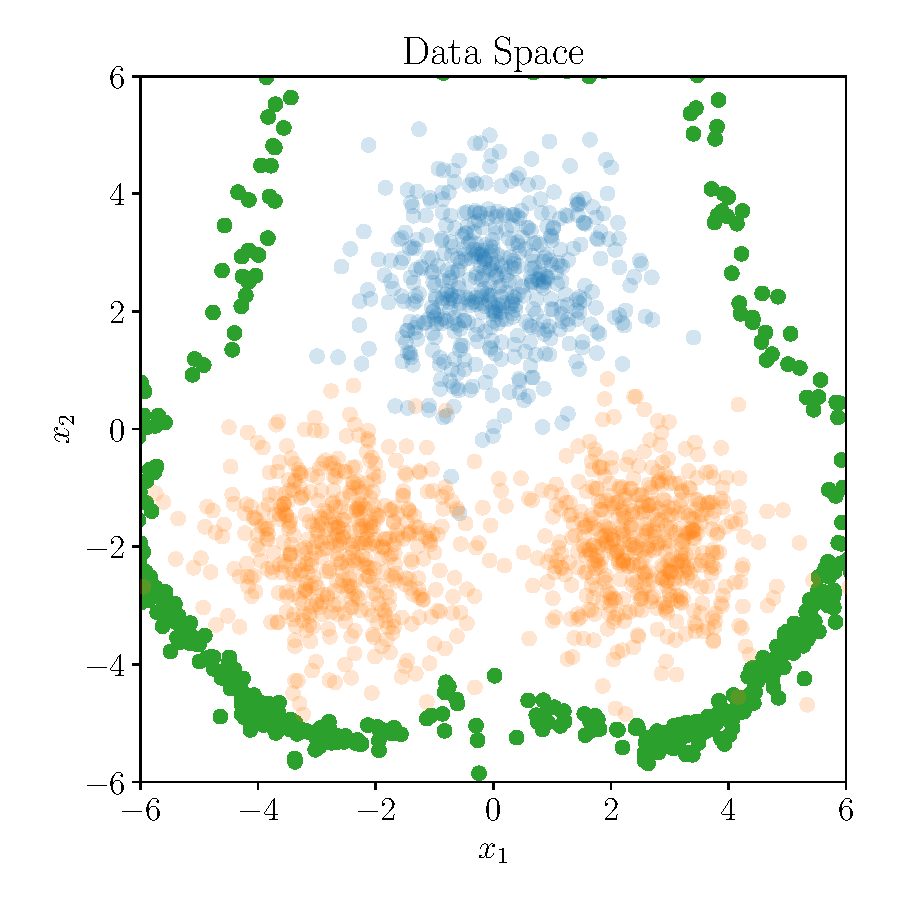
\includegraphics[width=\linewidth]{figures/toy_example/gaussian_mixture/gumbel_samples.pdf}
        \caption{Test}
        \label{fig:gmm_sample_space_gumbel}
    \end{subfigure}
    \begin{subfigure}[]{0.4\textwidth}
        \centering
    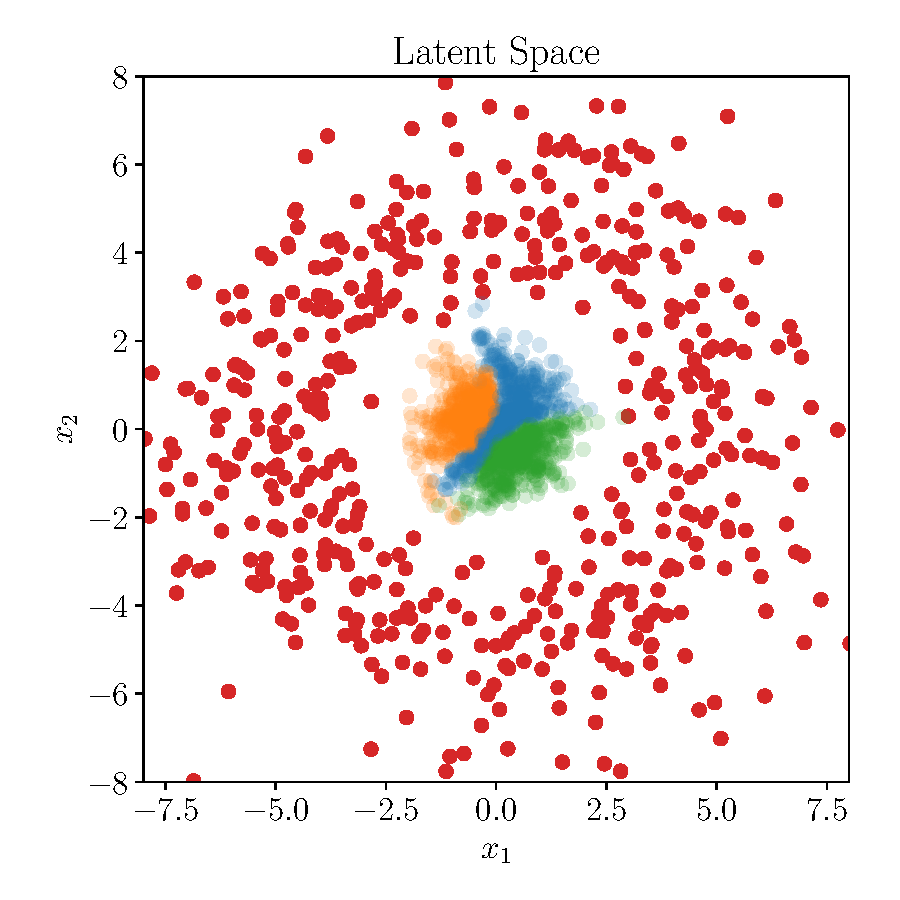
\includegraphics[width=\linewidth]{figures/toy_example/gaussian_mixture/latent_space_with_outliers.pdf}
        \caption{Test}
        \label{fig:gmm_latent_space_gumbel}
    \end{subfigure}
    \caption{Gaussian mixture latent mapping}%
    \label{fig:latent_gmm}
\end{figure}

\begin{figure}[htpb]
    \centering
    \begin{subfigure}[]{0.4\textwidth}
        \centering
    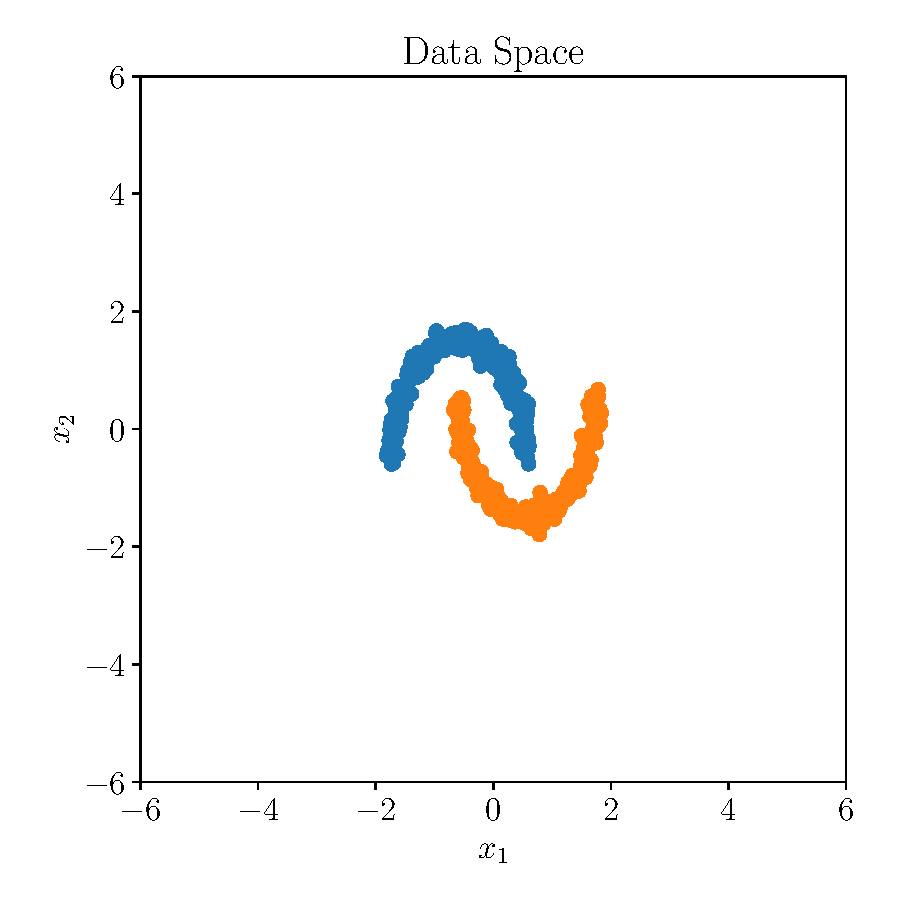
\includegraphics[width=\linewidth]{figures/toy_example/moons/toy_data.pdf}
        \caption{Test}
        \label{fig:moons_sample_space}
    \end{subfigure}
    \begin{subfigure}[]{0.4\textwidth}
        \centering
    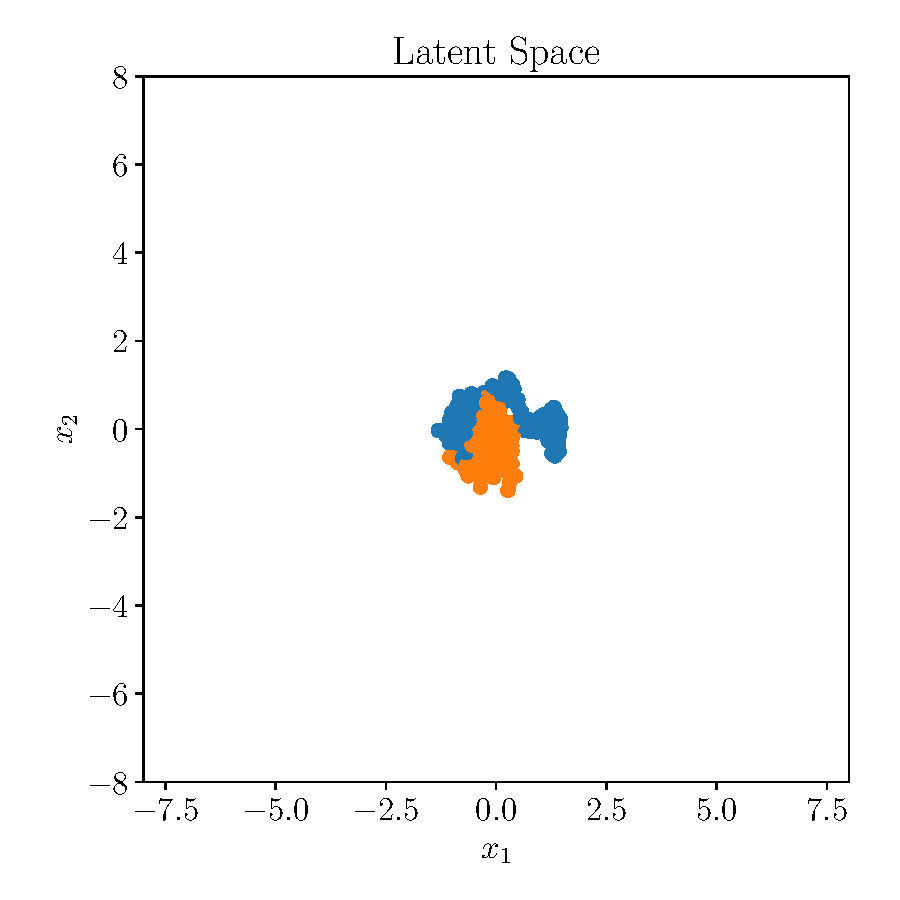
\includegraphics[width=\linewidth]{figures/toy_example/moons/latent_space.pdf}
        \caption{Test}
        \label{fig:moons_latent_space}
    \end{subfigure}
    \begin{subfigure}[]{0.4\textwidth}
        \centering
    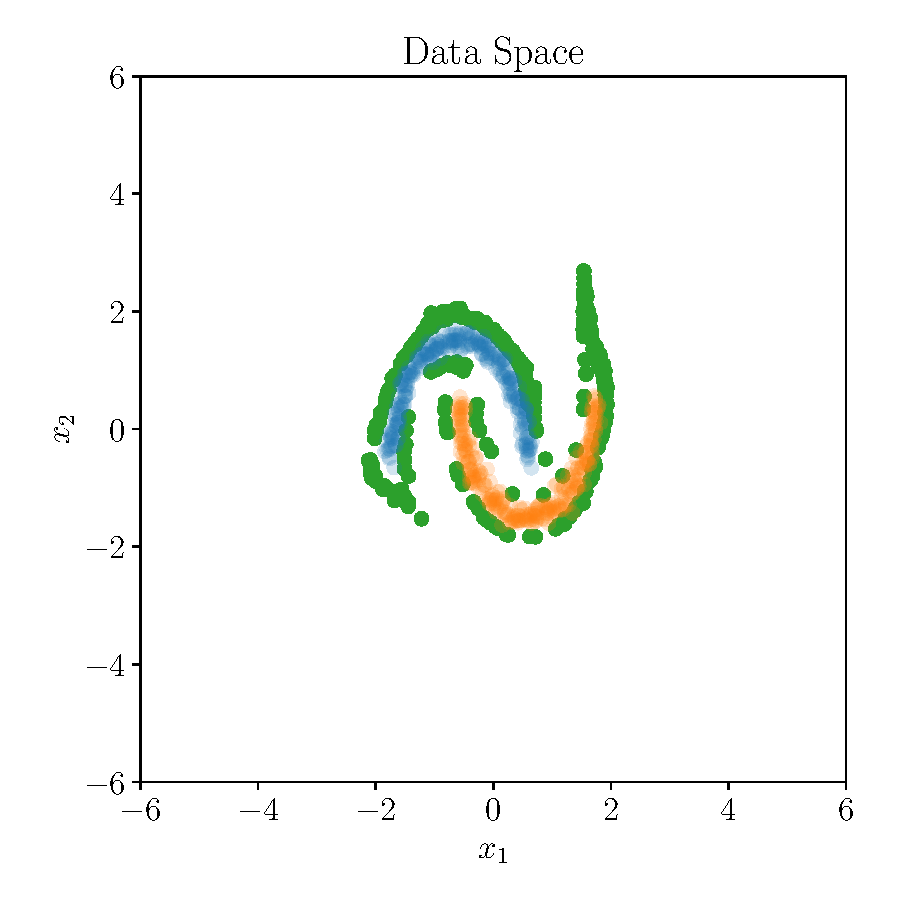
\includegraphics[width=\linewidth]{figures/toy_example/moons/gumbel_samples.pdf}
        \caption{Test}
        \label{fig:moons_sample_space_gumbel}
    \end{subfigure}
    \begin{subfigure}[]{0.4\textwidth}
        \centering
    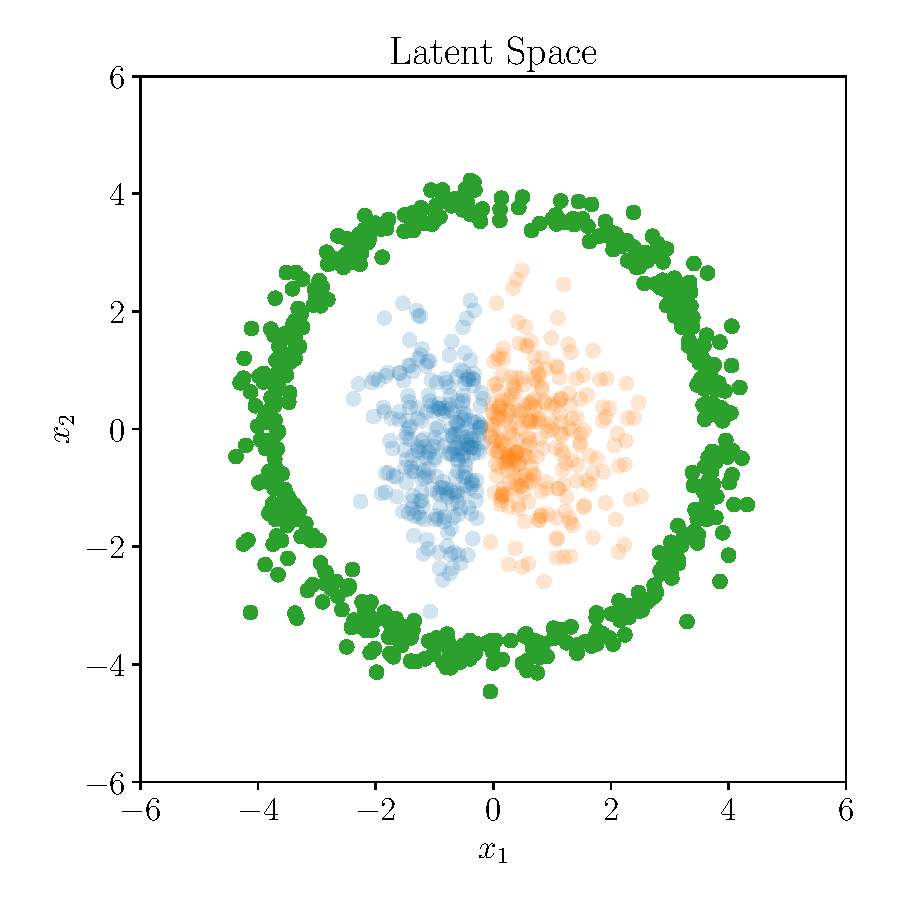
\includegraphics[width=\linewidth]{figures/toy_example/moons/latent_space_with_outliers.pdf}
        \caption{Test}
        \label{fig:moons_latent_space_gumbel}
    \end{subfigure}
    \caption{Moons latent mapping}%
    \label{fig:latent_moons}
\end{figure}

Let us first investigate our methods on some simple toy data. For this we
generate two toy datasets. One dataset consists of three two-dimensional
gaussian distributions, each being its own class. The other dataset has two
classes shaped like interlocked moons. Both datasets are normalized. On each
dataset we train a simple version of the normalizing flow introduced above. It
consists of three \textcolor{red}{TYPE} coupling blocks, where the coupling
functions are neural networks with five linear layers with rectified linear
units as activation functions. As described in
\autoref{sec:network_architecture} it is trained to maximize the likelihood of
the training data.

Samples from the gaussian mixture toy dataset can be seen in
\autoref{fig:gmm_sample_space}. The learned latent space for the gaussian
mixture toy dataset is shown in \autoref{fig:gmm_latent_space}. As we can see
the latent space approximates a standard normal distribution and each class
gets mapped to a region of this distribution.

For the moons toy dataset, samples can be seen in
\autoref{fig:moons_sample_space} and the learned latent space is shown in
\autoref{fig:moons_latent_space}. Again we observe a reasonable approximation
of a standard normal distribution in the latent space.

We can now take a look at the generation of outliers. Since the latent space is
low-dimensional we use the Gumbel distribution sampling as described in
\autoref{sub:gumbel_distribution}. \textcolor{red}{PARAMS}. The sampled ring in
the latent space can be seen in \autoref{fig:gmm_latent_space_gumbel} for the
gaussian mixture dataset and in \autoref{fig:moons_latent_space_gumbel} for the
moons dataset. Using the normalizing flow to transform the outlier samples back
to the data space we get samples that encase the inlier datas. For the gaussian
mixture dataset this can be seen in \autoref{fig:gmm_sample_space_gumbel} and
in \autoref{fig:moons_sample_space_gumbel} for the moons dataset.

\begin{figure}[htpb]
    \centering
    \begin{subfigure}[]{0.4\textwidth}
        \centering
        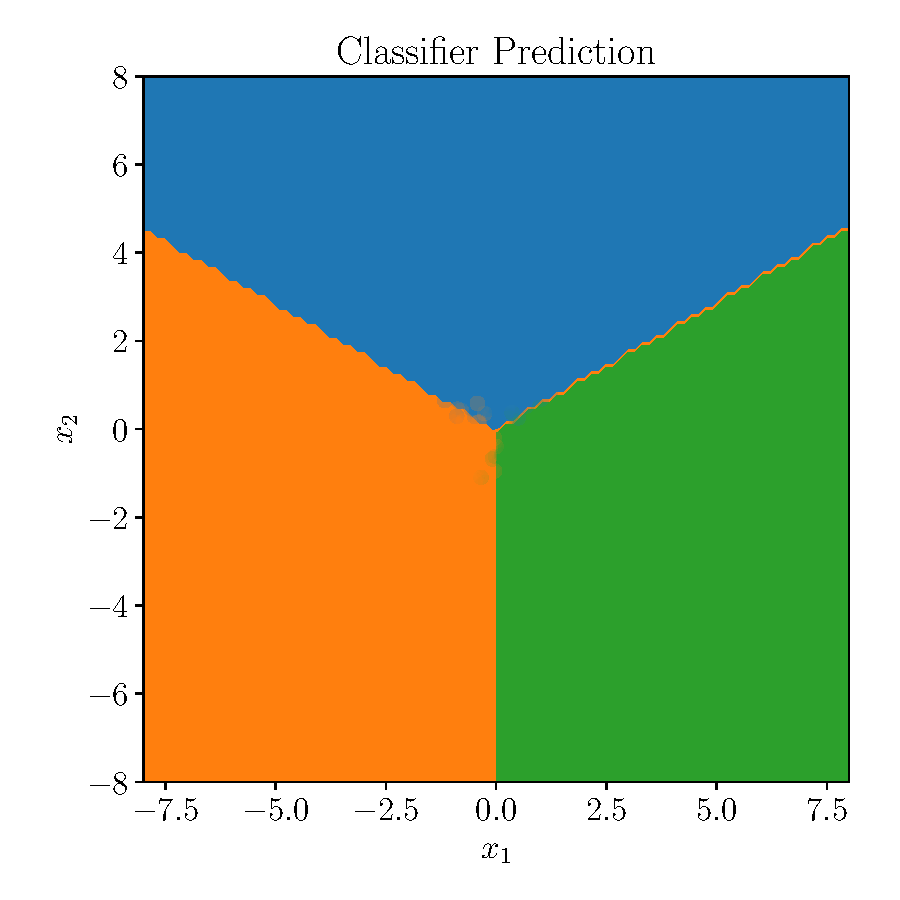
\includegraphics[width=\linewidth]{figures/toy_example/gaussian_mixture/classifier_class.pdf}
        \caption{Test}
        \label{fig:gmm_class}
    \end{subfigure}
    % \hfill
    \begin{subfigure}[]{0.4\textwidth}
        \centering
        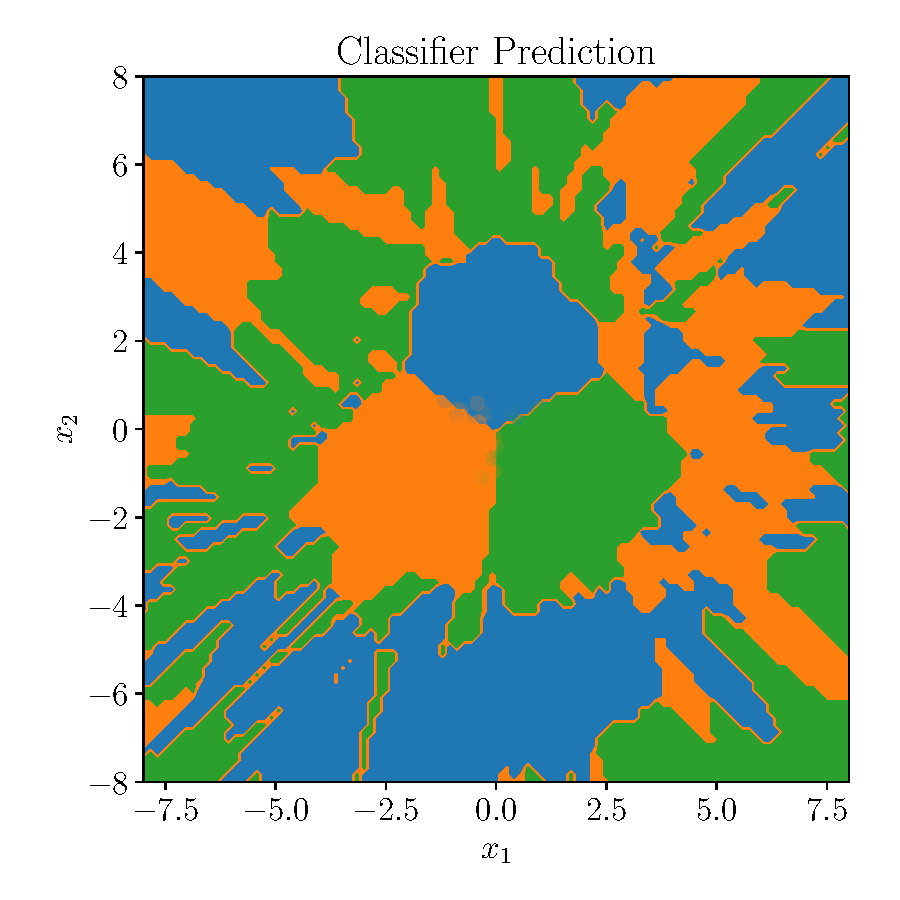
\includegraphics[width=\linewidth]{figures/toy_example/gaussian_mixture/classifier_kl_class.pdf}
        \caption{Test}
        \label{fig:gmm_class_kl}
    \end{subfigure}
    \begin{subfigure}[]{0.4\textwidth}
        \centering
    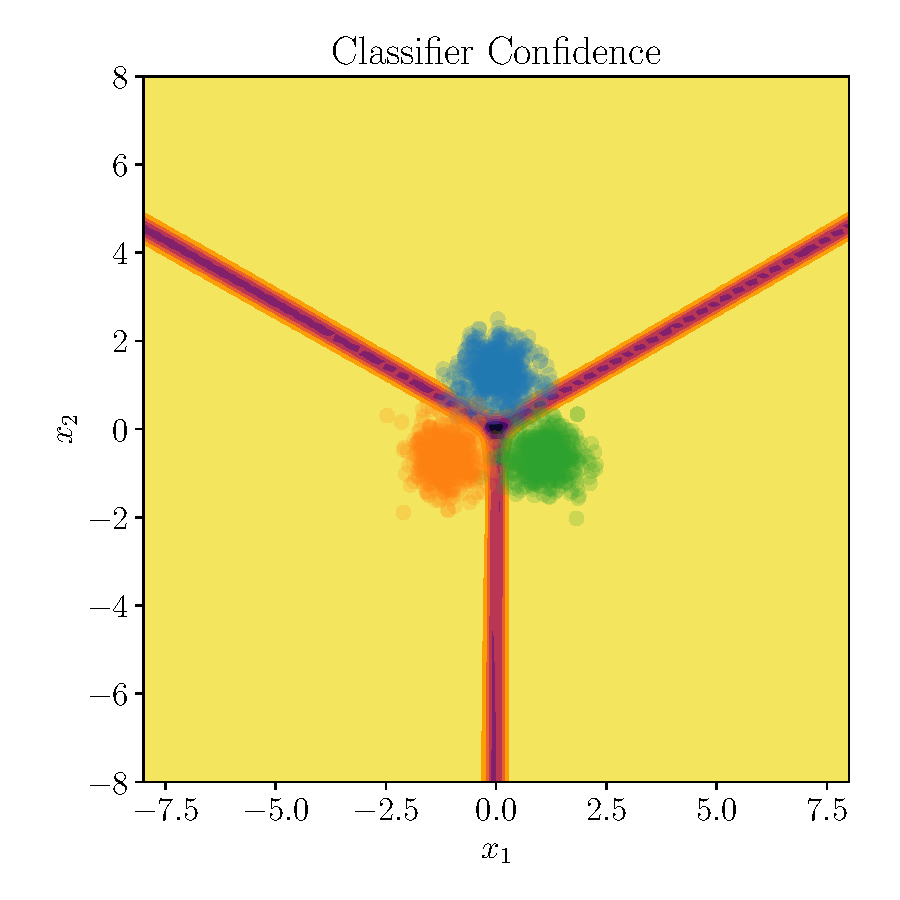
\includegraphics[width=\linewidth]{figures/toy_example/gaussian_mixture/classifier_confidence.pdf}
        \caption{Test}
        \label{fig:gmm_confidence}
    \end{subfigure}
    \begin{subfigure}[]{0.4\textwidth}
        \centering
    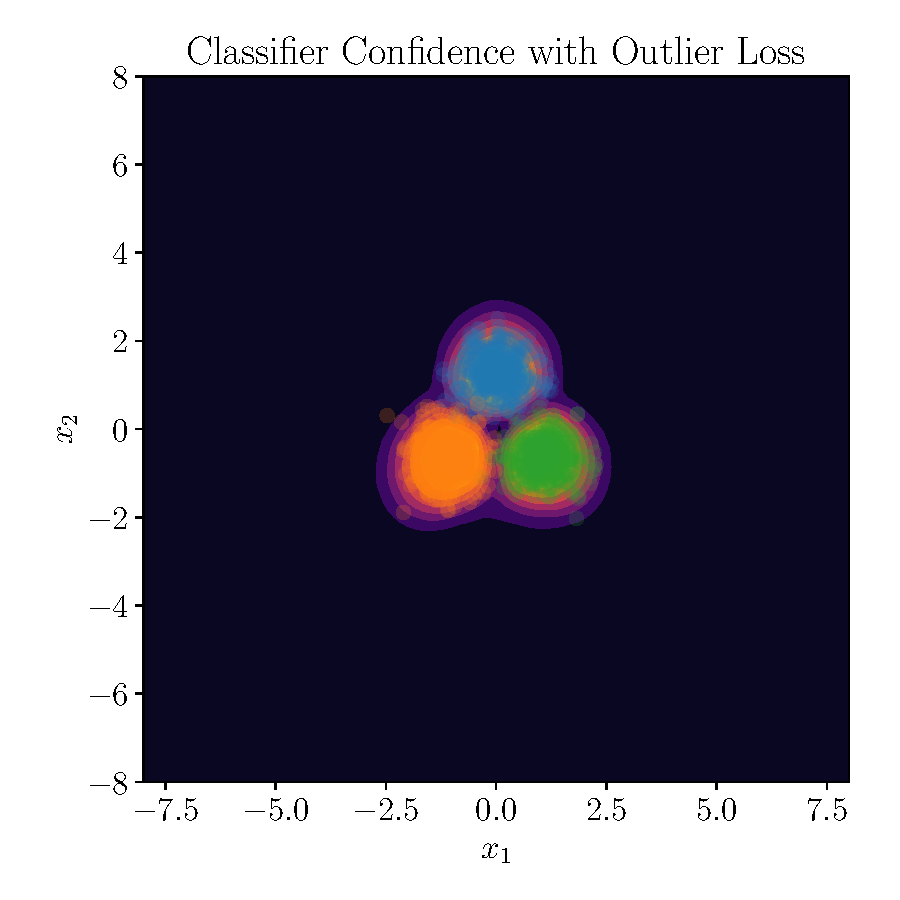
\includegraphics[width=\linewidth]{figures/toy_example/gaussian_mixture/classifier_kl_confidence.pdf}
        \caption{Test}
        \label{fig:gmm_confidence_kl}
    \end{subfigure}
    
    \caption{Gaussian mixture classifier performance}%
    \label{fig:classifier_gmm}
\end{figure}

\begin{figure}[htpb]
    \centering
    \begin{subfigure}[]{0.4\textwidth}
        \centering
        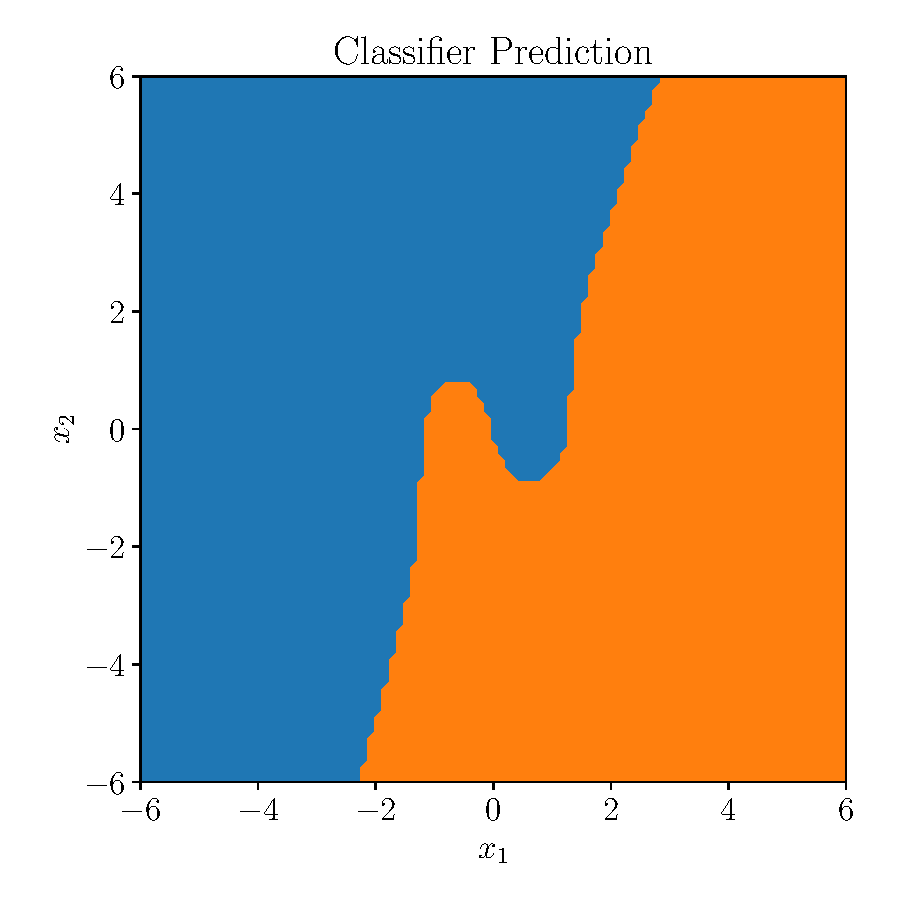
\includegraphics[width=\linewidth]{figures/toy_example/moons/classifier_class.pdf}
        \caption{Test}
        \label{fig:moons_class}
    \end{subfigure}
    % \hfill
    \begin{subfigure}[]{0.4\textwidth}
        \centering
        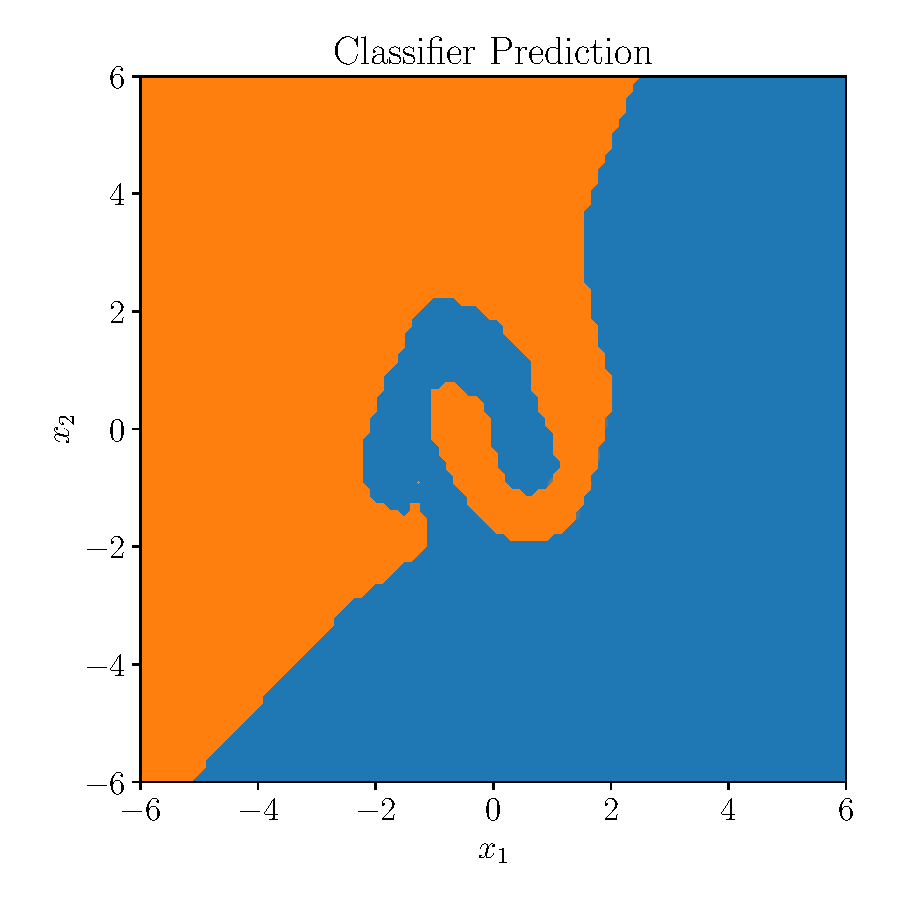
\includegraphics[width=\linewidth]{figures/toy_example/moons/classifier_kl_class.pdf}
        \caption{Test}
        \label{fig:moons_class_kl}
    \end{subfigure}
    \begin{subfigure}[]{0.4\textwidth}
        \centering
    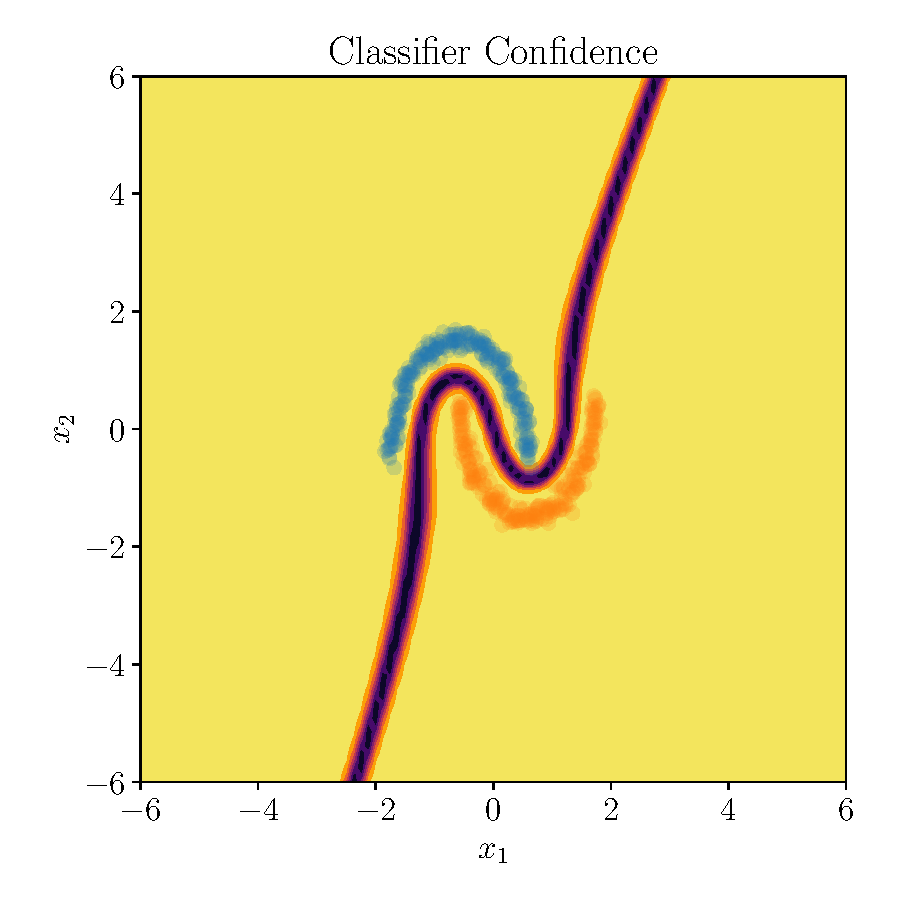
\includegraphics[width=\linewidth]{figures/toy_example/moons/classifier_confidence.pdf}
        \caption{Test}
        \label{fig:moons_confidence}
    \end{subfigure}
    \begin{subfigure}[]{0.4\textwidth}
        \centering
    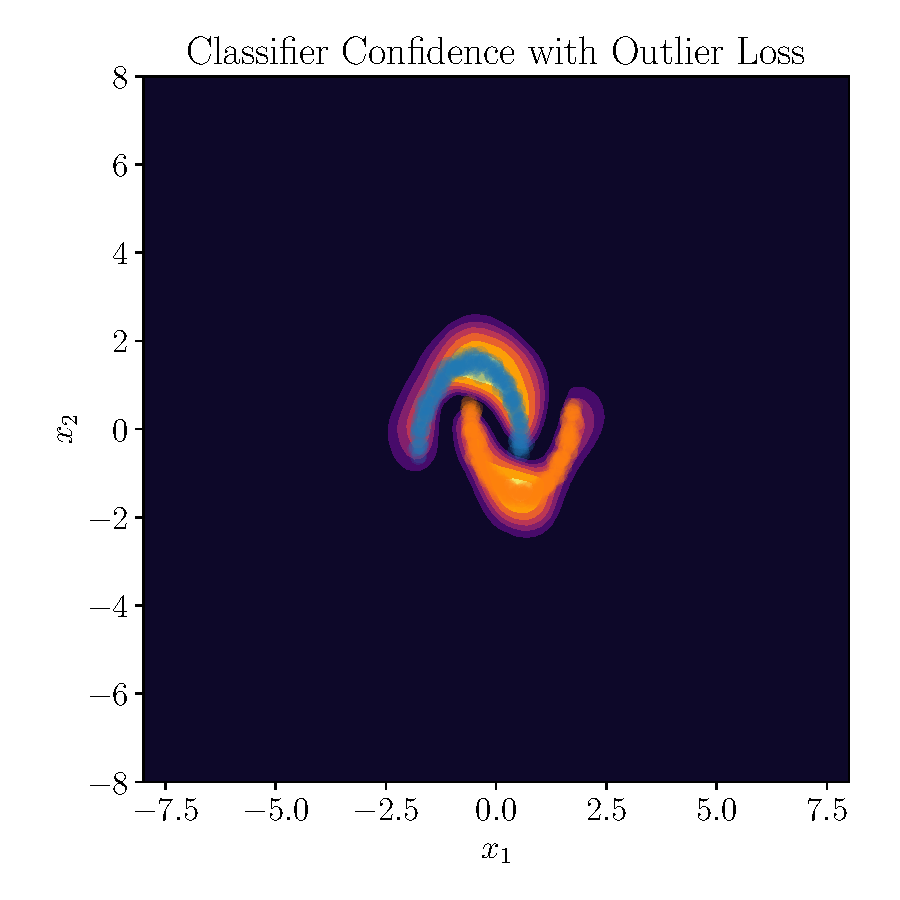
\includegraphics[width=\linewidth]{figures/toy_example/moons/classifier_kl_confidence.pdf}
        \caption{Test}
        \label{fig:moons_confidence_kl}
    \end{subfigure}
    
    \caption{Moons classifier performance}%
    \label{fig:classifier_moons}
\end{figure}

To show how the generated outliers can be of use we can train a classifier on
the toy datasets. The classifier is a simple neural network consisting of three
linear layers with rectified linear units as activations. It is trained on the
generated data to minimize the cross-entropy between the ground truth labels
and the predicted labels. This simple setup leads to a classifier that
performes well on both datasets, the decision regions can be seen in
\autoref{fig:gmm_class} and \autoref{fig:moons_class} respectively. To get a
measure of the confidence of the classifier we can inspect the entropy of the
predicted class distribution. We can see in \autoref{fig:gmm_confidence} and
\autoref{fig:moons_confidence}, that this classifier has high confidence
everywhere except in a small boundary region between the classes. This is often
undesired, as this means outliers remain undetected and receive a oftentimes
wrong class prediction. 

This can be mitigated by augmenting the loss of the classifier as described in
\autoref{sec:discriminator_training}. We train the classifier to minimize the
Kullback-Leibler divergence between the predicted class distribution and a
uniform class distribution over the generated outliers. As we can see in
\autoref{fig:gmm_confidence_kl} and \autoref{fig:moons_confidence_kl} this
leads to regions of low confidence all around the data regions while keeping
good decision boundaries in the region of high confidence, shown in
\autoref{fig:gmm_class_kl} and \autoref{fig:moons_class_kl}.

\section{Qualitative Comparison}%
\label{sec:qualitative_comparison}

\begin{figure}[htpb]
    \centering
    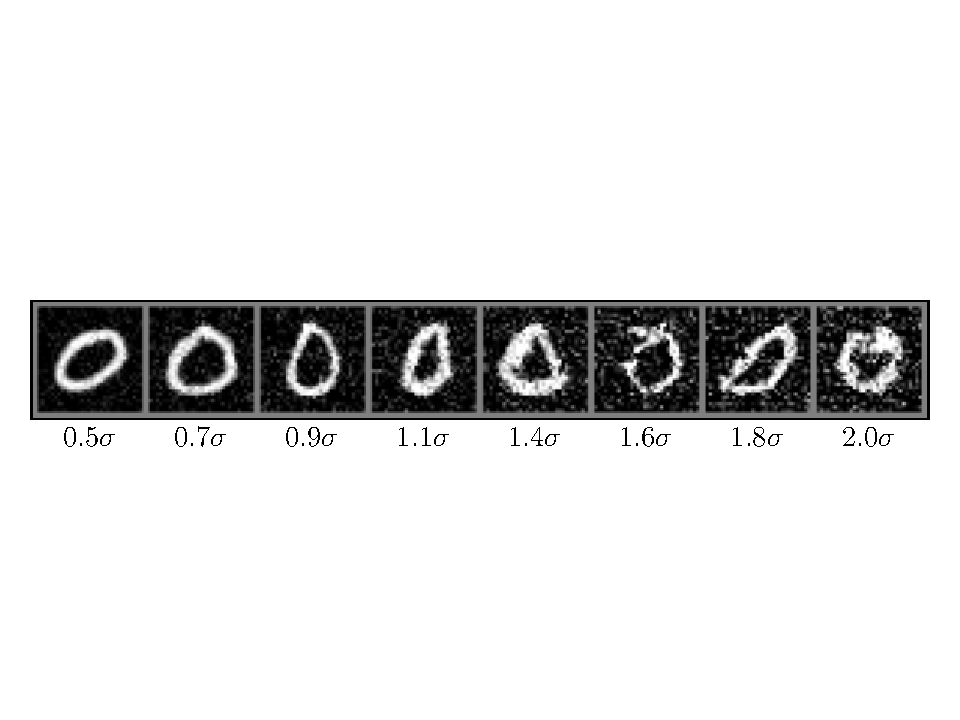
\includegraphics[width=0.8\linewidth]{figures/samples/emnist_inc_distance.pdf}
    \caption{}%
    \label{fig:}
\end{figure}

\begin{figure}[htpb]
    \centering
    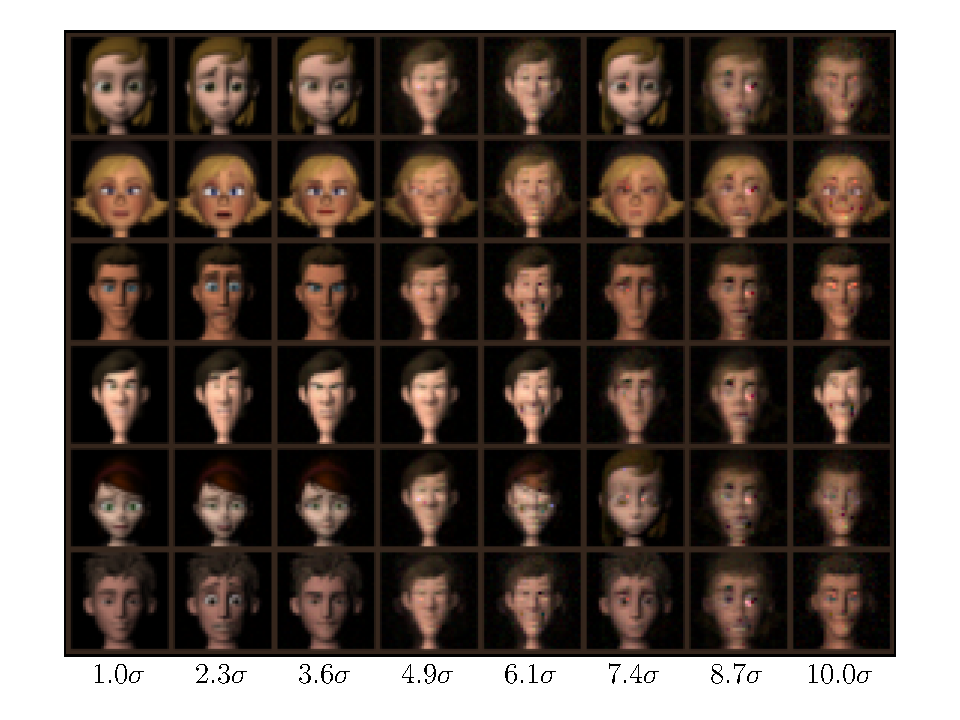
\includegraphics[width=0.8\linewidth]{figures/samples/ferg_people_inc_distance.pdf}
    \caption{}%
    \label{fig:}
\end{figure}

\subsection{Archetypal Analysis}%
\label{sub:archetypal_analysis}

\begin{figure}[htpb]
    \centering
    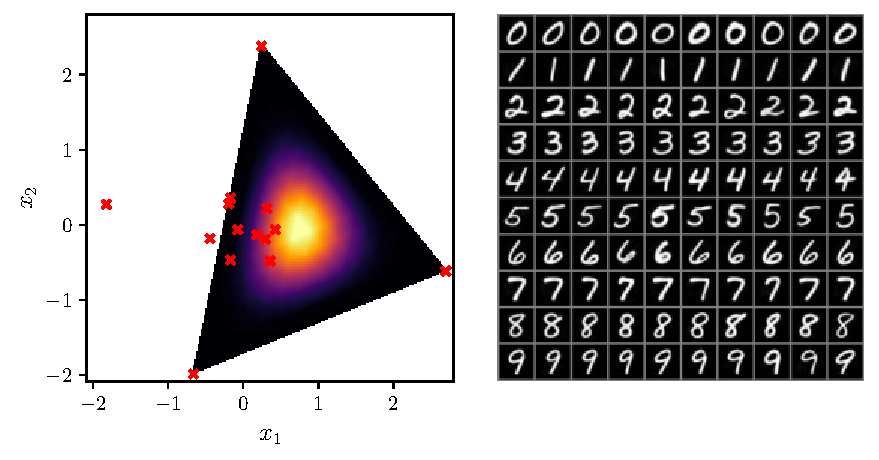
\includegraphics[width=1\linewidth]{figures/samples/aa_emnist.pdf}
    \caption{AA FERG}%
    \label{fig:aa_emnist}
\end{figure}

\begin{figure}[htpb]
    \centering
    \begin{subfigure}[htpb]{\textwidth}
        \centering
        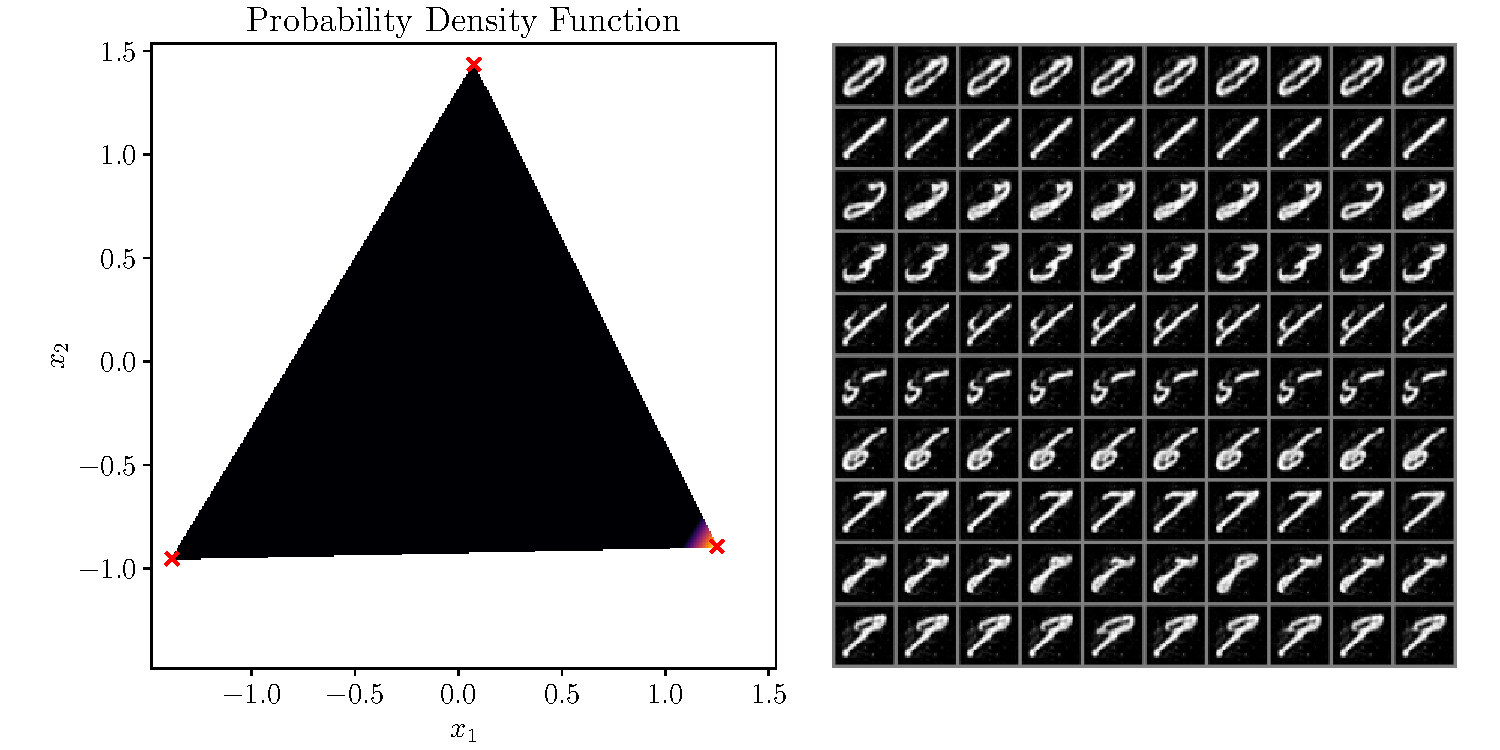
\includegraphics[width=1\linewidth]{figures/samples/aa_emnist1.pdf}
    \end{subfigure}

    \begin{subfigure}[htpb]{\textwidth}
        \centering
        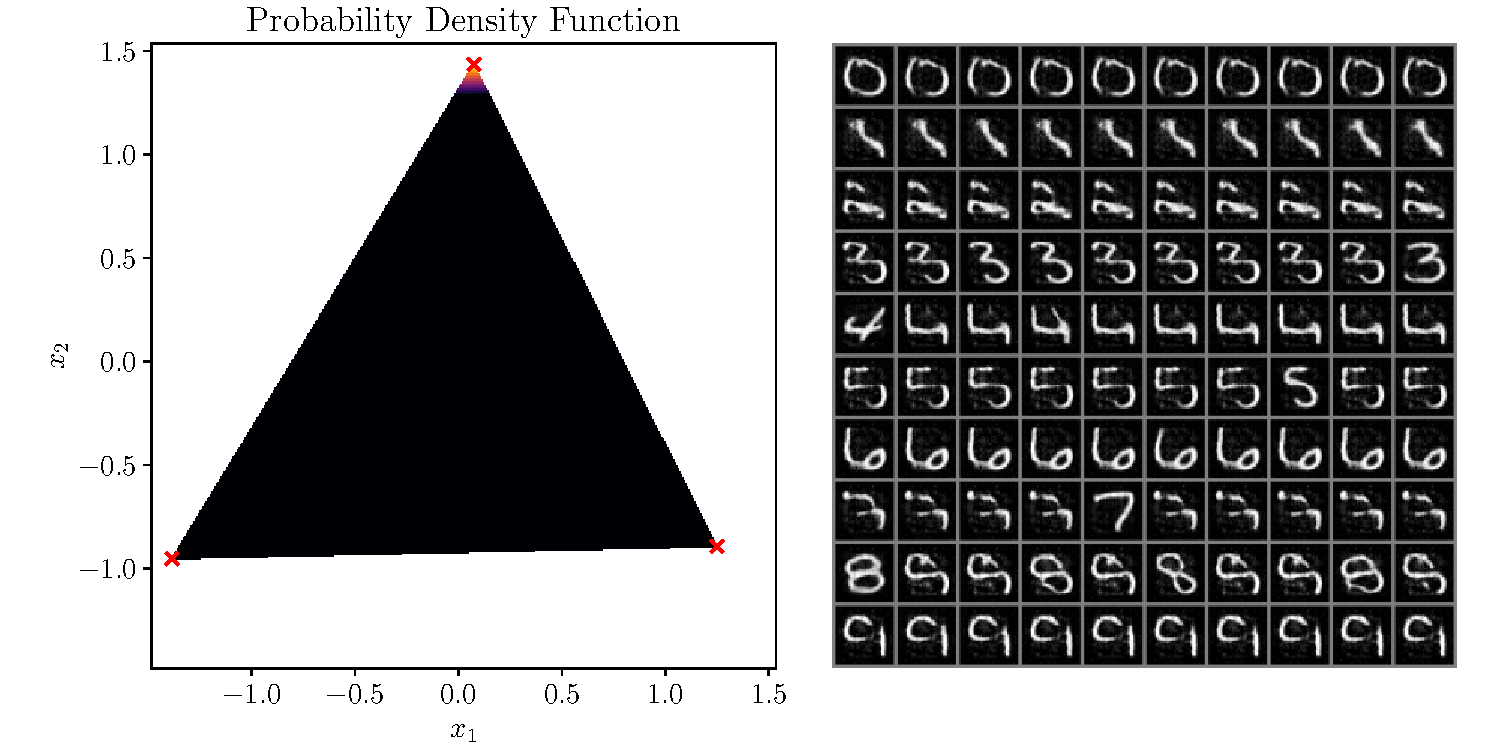
\includegraphics[width=1\linewidth]{figures/samples/aa_emnist2.pdf}
    \end{subfigure}

    \begin{subfigure}[htpb]{\textwidth}
        \centering
        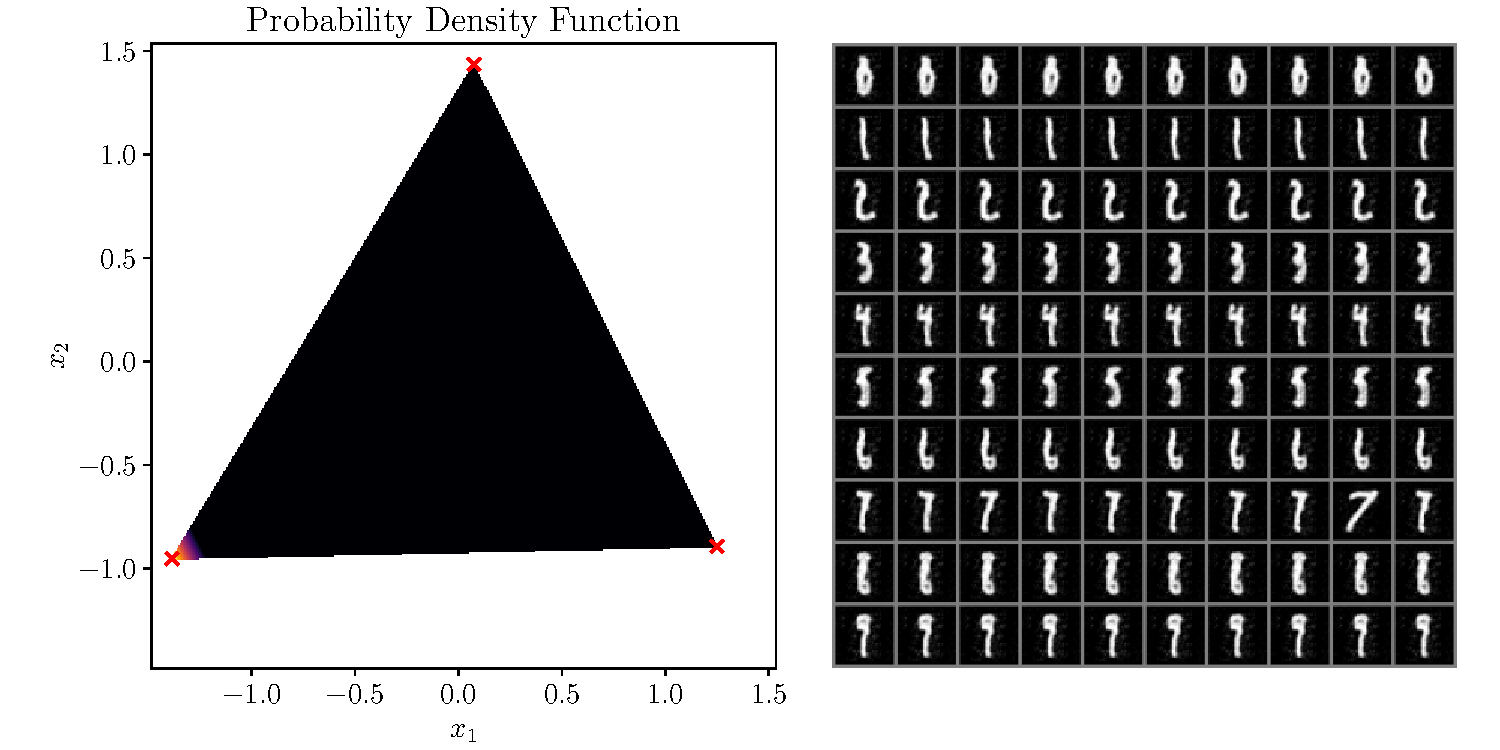
\includegraphics[width=1\linewidth]{figures/samples/aa_emnist3.pdf}
    \end{subfigure}
    \caption{Name}%
    \label{fig:aa_emnist_corners}
\end{figure}

\begin{figure}[htpb]
    \centering
    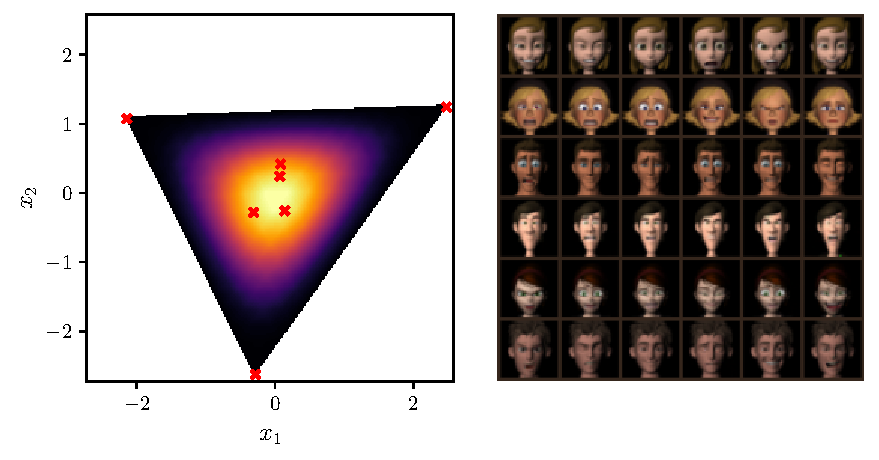
\includegraphics[width=1\linewidth]{figures/samples/aa_ferg.pdf}
    \caption{AA FERG}%
    \label{fig:aa_ferg}
\end{figure}

\begin{figure}[htpb]
    \centering
    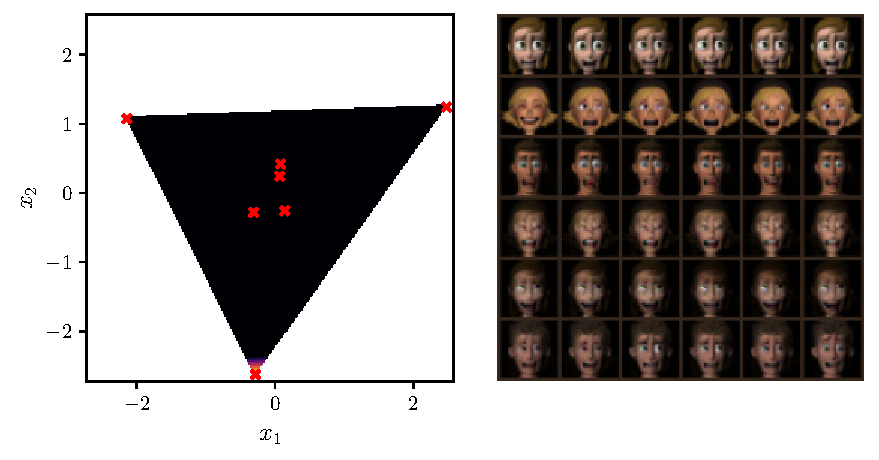
\includegraphics[width=1\linewidth]{figures/samples/aa_ferg1.pdf}
    \caption{AA FERG}%
    \label{fig:aa_ferg}
\end{figure}

\begin{figure}[htpb]
    \centering
    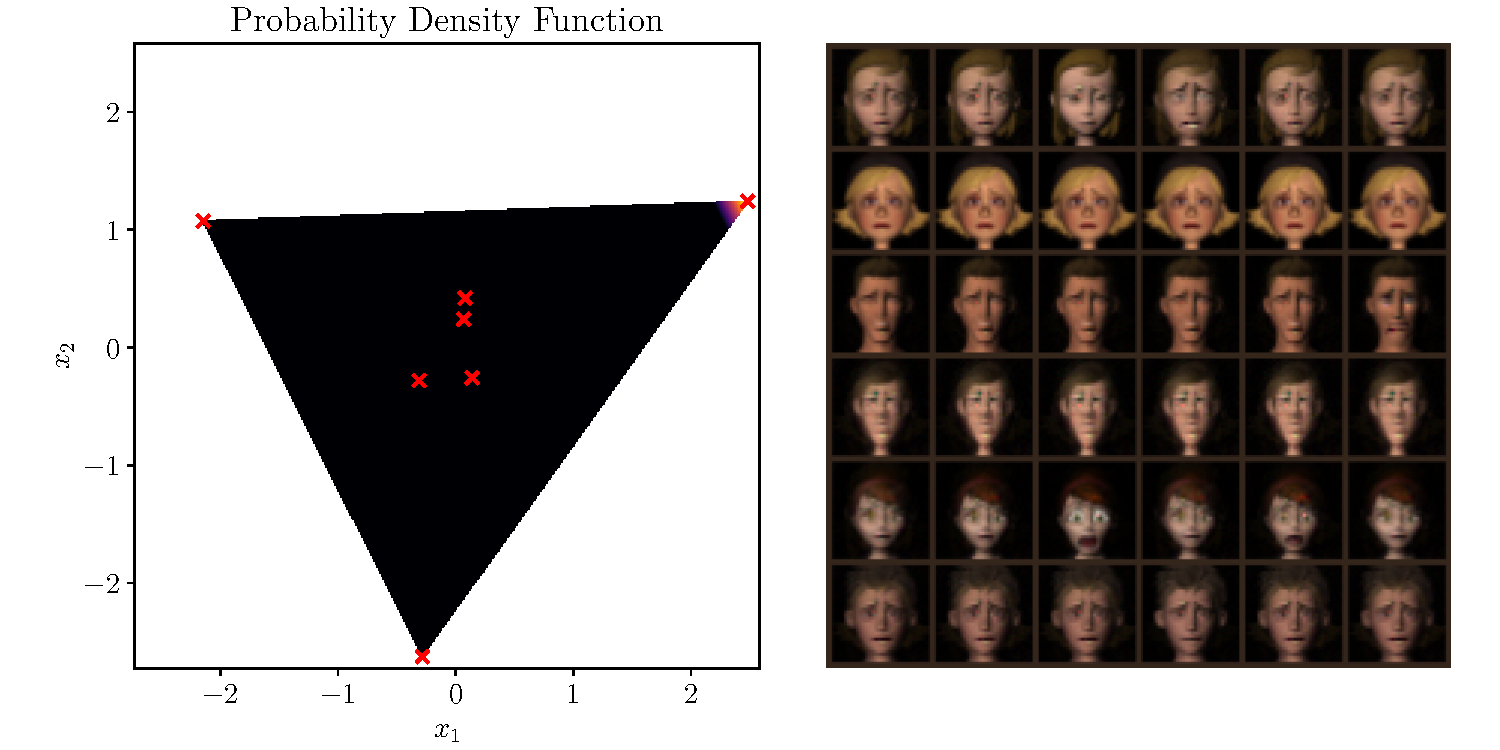
\includegraphics[width=1\linewidth]{figures/samples/aa_ferg2.pdf}
    \caption{AA FERG}%
    \label{fig:aa_ferg}
\end{figure}

\begin{figure}[htpb]
    \centering
    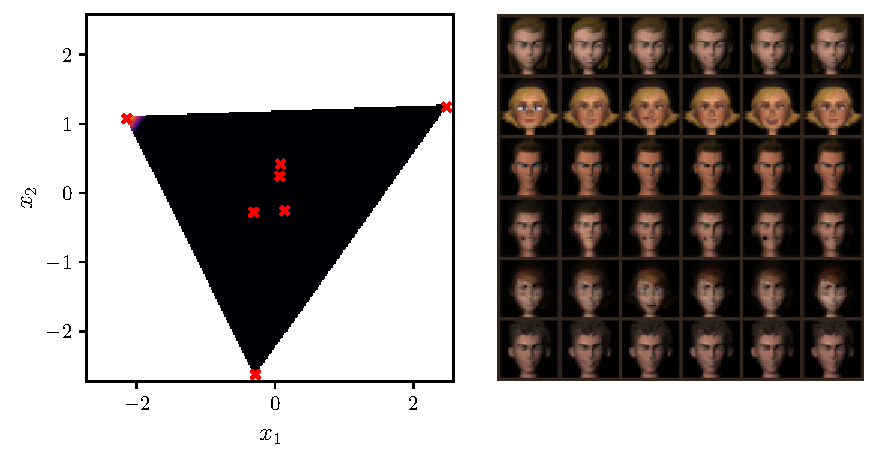
\includegraphics[width=1\linewidth]{figures/samples/aa_ferg3.pdf}
    \caption{AA FERG}%
    \label{fig:aa_ferg}
\end{figure}

\begin{figure}[htpb]
    \centering
    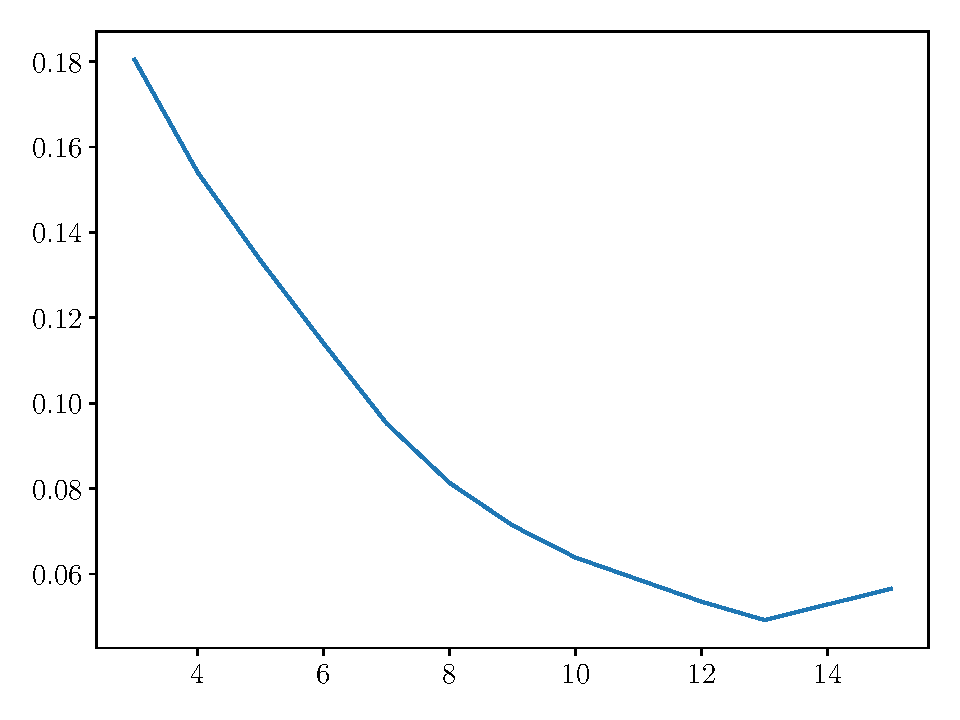
\includegraphics[width=0.8\linewidth]{figures/samples/emnist_aa_mse_na.pdf}
    \caption{}%
    \label{fig:emnist_aa_mse}
\end{figure}


\section{Analysis of the Latent Space}%
\label{sec:analysis_of_the_latent_space}

\begin{figure}[htpb]
    \centering
    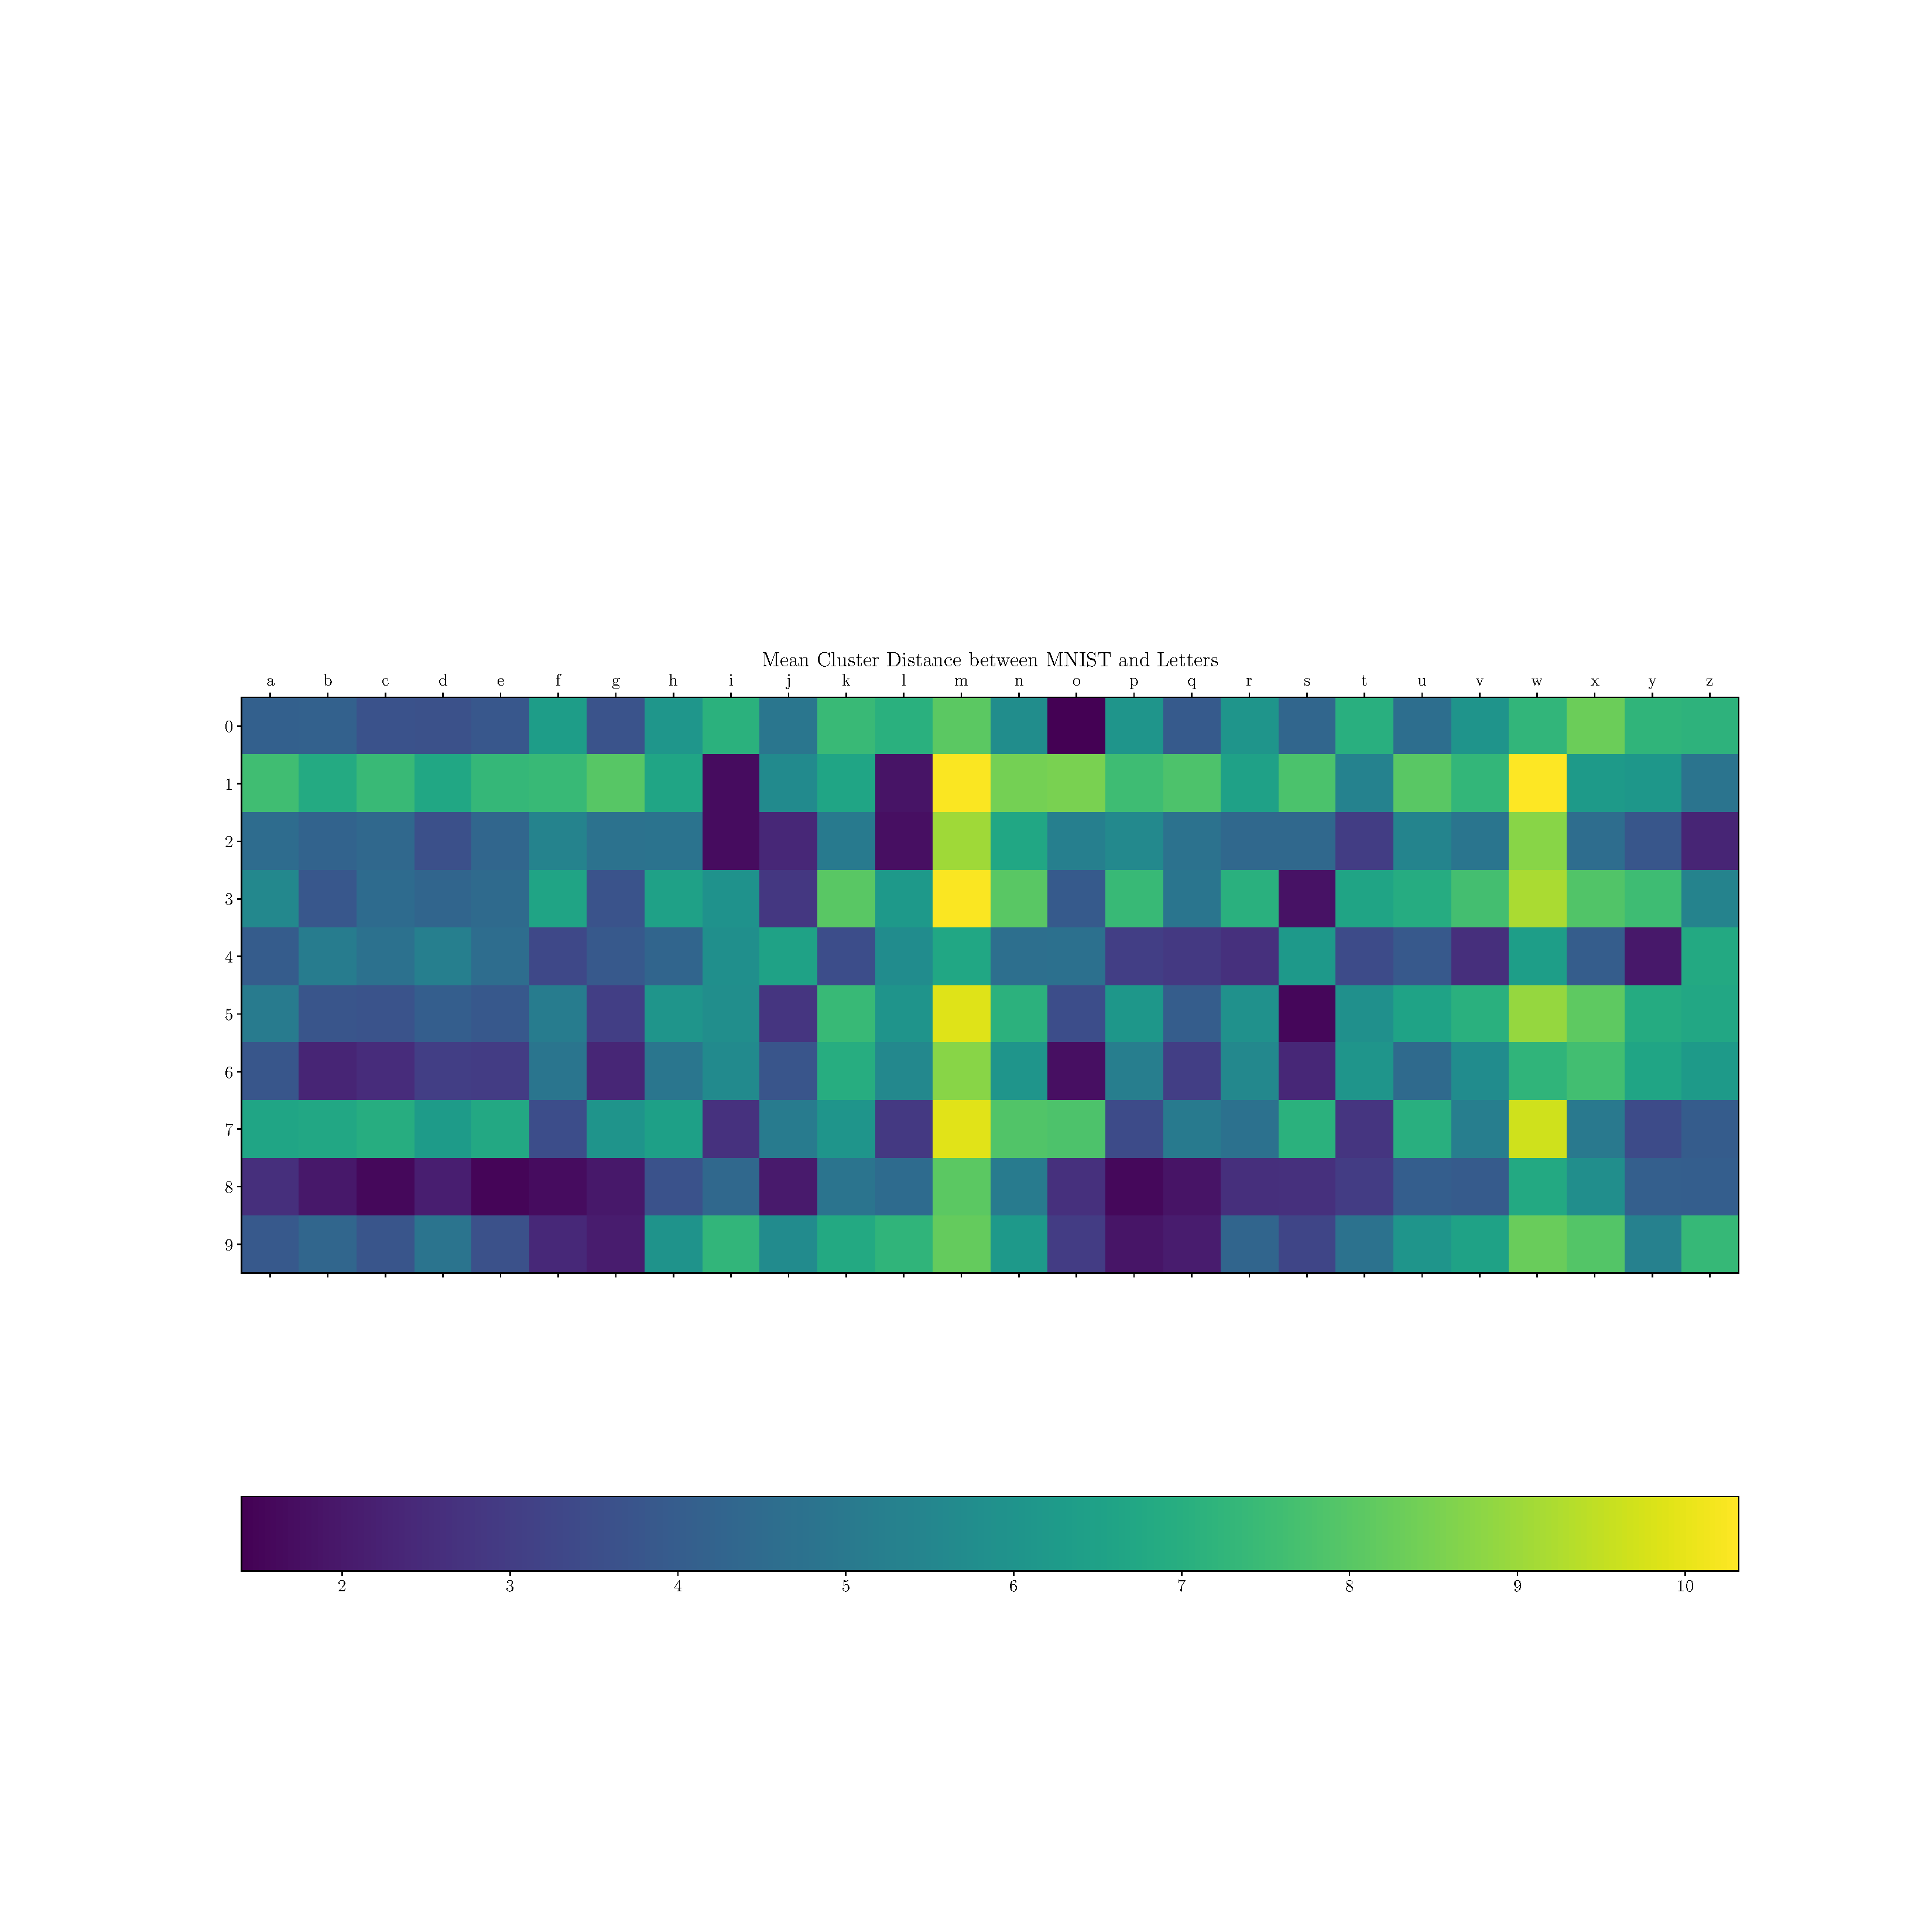
\includegraphics[width=0.8\linewidth]{figures/samples/emnist_distance_matrix_letters.pdf}
    \caption{}%
    \label{fig:}
\end{figure}

\begin{figure}[htpb]
    \centering
    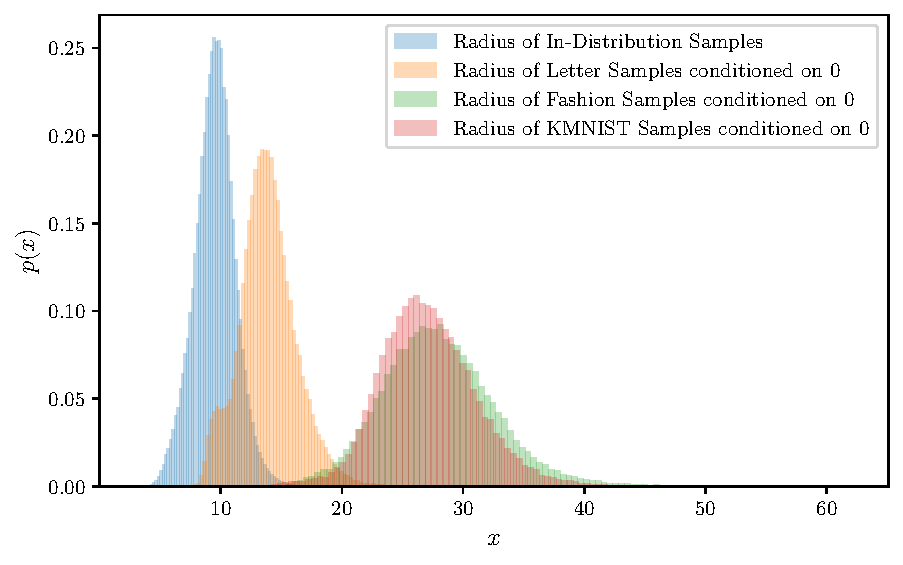
\includegraphics[width=0.8\linewidth]{figures/samples/emnist_radius_hist.pdf}
    \caption{}%
    \label{fig:}
\end{figure}


\section{Discriminator Performance}%
\label{sec:discriminator_performance}


\section{General Performance}%
\label{sec:general_performance}

% What did I even mean by this?

\section{Robustness}%
\label{sec:robustness}

% If there is time for this

% TODO: Check if anything Ulli requested isn't done yet %
